\documentclass{article}
\renewcommand{\baselinestretch}{1.25}
% \usepackage[
% a4paper,landscape,
% total={284mm,170mm},
% bottom=7mm,
% top=14mm,headsep=3mm]{geometry}
\usepackage[utf8]{inputenc}
\usepackage[T1]{fontenc}
\usepackage{textcomp}
\usepackage{amsmath, amssymb, amsthm}
% \usepackage[outputdir=tmp]{minted}
% \usepackage{lmodern}
\usepackage{multicol}
% \setlength{\columnsep}{4mm}
\usepackage{fancyhdr}
\usepackage{lastpage}
\usepackage{tikz}
\usepackage{pgfplots, pgfplotstable}
\usetikzlibrary{quotes,angles}
% \pagestyle{fancy}
% \fancyhf{}
% \rhead{Page \thepage/\pageref{LastPage}}
% \lhead{Made by Tan Yee Jian (\texttt{@swampertx})}
% \chead{MA2108S Cheat Sheet}

% figure support
\usepackage{import}
\usepackage{xifthen}
\pdfminorversion=7
\usepackage{pdfpages}
\usepackage{transparent}
% \newcommand{\incfig}[1]{
% \def\svgwidth{\columnwidth}
% import{./}{#1}
% }
\usepackage{arcs}
\usepackage{graphicx}
\graphicspath{ {./} }

\pdfsuppresswarningpagegroup=1

\newtheorem{thm}{Theorem}[section]
\newtheorem{crl}{Corollary}[thm]
\newtheorem*{lemma}{Lemma}
\newtheorem{note}{Note}[thm]
\newtheorem{defn}{Definition}[section]
\newtheorem{ex}{Example}[section]
\newtheorem{prop}{Proposition}[section]
\newtheorem{obs}{Observation}
\newtheorem*{claim}{Claim}

\newcommand{\pmat}[1]{ \begin{pmatrix}#1\end{pmatrix} }
\newcommand{\seqn}[1]{(#1)^\infty_{n=1}}
\newcommand{\seqk}[1]{(#1)^\infty_{k=1}}
% (series term): returns a series with counter n=1 to \infty.
\newcommand{\infsrsn}[1]{\sum\limits^\infty_{n=1}#1}
\newcommand{\infsrsk}[1]{\sum\limits^\infty_{k=1}#1}
\newcommand{\real}{\mathbb{R}}
\newcommand{\nat}{\mathbb{N}}
\newcommand{\rat}{\mathbb{Q}}
\newcommand{\cmm}{C(M_1,M_2)}
\newcommand{\met}[1]{\langle M_{#1},\rho_{#1}\rangle}
\newcommand{\ntoinf}{\limits_{n\to\infty}}
\newcommand{\ktoinf}{\limits_{k\to\infty}}
% \newcommand{\onetoinf}[]{^\infty_{n=1}}
\newcommand{\limn}[1]{\lim\ntoinf #1}
\newcommand{\limk}[1]{\lim\ktoinf #1}

\DeclareMathOperator{\spn}{span}
\DeclareMathOperator{\diam}{diam}


\title{UNL2210 Homework 1}
\author{Group 9: Keane, Pei Han, Yee Jian}
\date{\today}

\begin{document}
\maketitle
\section*{Question 7}
\pgfplotstableread{
  X Y
40.9 128.5
40 125.5
36.8 115.8
33.8 106.4
30.9 97.2
27.9 87.8
26.9 84.7
26 81.6
23 72.1
20.8 65.7
19 59.6
15.9 50
}\datatable

% \begin{tikzpicture}
% \begin{axis}[legend pos=outer north east]
% \addplot [only marks, mark = *] table {\datatable};
% \addplot [thick, red] table[
%     y={create col/linear regression={y=Y}}
% ] % compute a linear regression from the input table
% {\datatable};
% \addlegendentry{$y(x)$}
% \addlegendentry{%
% $\pgfmathprintnumber{\pgfplotstableregressiona} \cdot x
% \pgfmathprintnumber[print sign]{\pgfplotstableregressionb}$}
% \end{axis}
% \end{tikzpicture}
\begin{centering}
\includegraphics{bfl.jpg}
\end{centering}
\section*{Question 8}
The statement that the ratio of the diameter to the circumference of any circle
is a constant is a synthetic a priori statement. It is a priori as it can be
proven from the axioms of Euclidean geometry and must be true for any circle.

A circle is a figure bounded by all points a constant length away from a fixed
point. As such, any two circles must be similar to each other, and the ratio of
their diameters must be equal to the ratio of their circumferences, ie.
$C_{1}/C_{2} = D_{1}/D_{2}$

Then $C_{1}/C_{2} = D_{1}/D_{2}$ for any two circles, and we call this constant ratio the
number $\pi$.

At the same time, the statement is also synthetic; the nature of the proposition
is not encapsulated in the definition of a circle. The deductive steps of
reasoning as mentioned above assume the use of Euclidean planes. Where there are
non-Euclidean planes, the ratio of circumference over diameter ($\pi$) may no
longer hold constant for all circles. The statement synthesises the concept of
circles (geometric constructs) with the notion of a "measure" and its
accompanying algebraic rules. It asserts more of the circle than what can
already be found in its definition.

\section*{Question 9}

\begin{center}
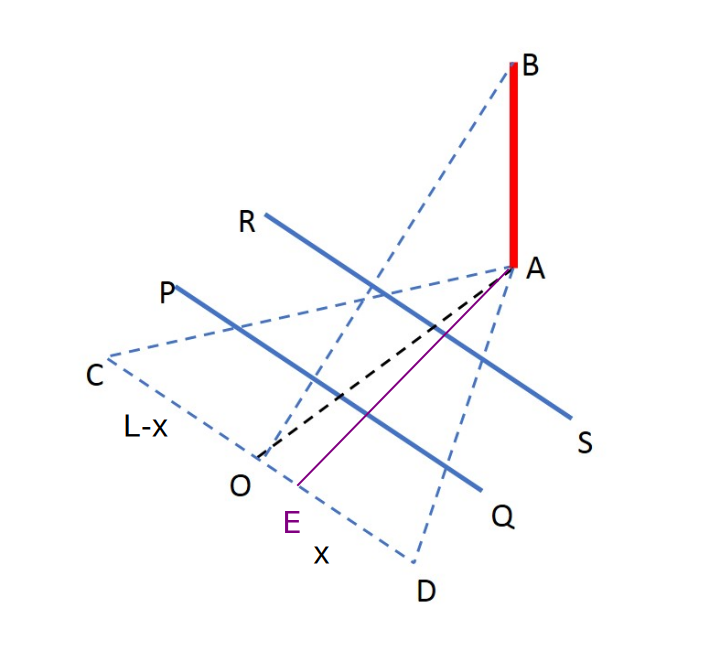
\includegraphics[width=8.5cm]{q9.png}
\end{center}
\begin{lemma}
\[AD=\frac{L\tan\beta}{(\tan\beta+\tan\alpha)\cos\alpha}\]
\end{lemma}
\begin{proof}
  As the figure above, let $E$ be the foot of perpendicular of $A$ on $CD$ such
  that $AE$ is perpendicular to $CD$. Let $DE=x,CE=L-x$. Now considering the
  right-angled triangle $AEC$,
  \[ AE = (L-x)\tan\beta\]
  and considering the right-angled triangle $AED$,
  \[ AE = x\tan\alpha\].
  Equating both, we have
  \begin{align*}
    (L-x)\tan\beta &= x\tan\alpha\\
    L\tan\beta &= x\tan\beta+x\tan\alpha\\
    x &= \frac{L\tan\beta}{\tan\beta+\tan\alpha}
  \end{align*}. Since $x/AD=\cos\alpha$, we must have
  \[ AD = \frac{x}{\cos\alpha} = \frac{L\tan\beta}{(\tan\beta+\tan\alpha)\cos\alpha}\]
  as desired.
\end{proof}
Now we show
\begin{align*}
  H &= \frac{L\tan\beta}{(\tan\beta+\tan\alpha)}\cdot\frac{\tan\gamma}{\cos\alpha}\\
  R &= \frac{L\tan\beta}{(\tan\beta+\tan\alpha)}\cdot\frac{1}{\cos\alpha}
\end{align*}
\begin{proof}
  First, notice that $H=AB$ is opposite $\angle BAD=\gamma$ in triangle
  $\triangle ABD$, thus
  \[H=AB=AD\cdot\tan\gamma= \frac{L\tan\beta}{(\tan\beta+\tan\alpha)}\cdot\frac{\tan\gamma}{\cos\alpha}\]
  and $R=AD$ is the other side in triangle $\triangle ABD$, the adjacent side of $\angle BAD$:
  \[ R=AD=\frac{AB}{\tan\angle BAD} = \frac{H}{\tan\gamma} = \frac{L\tan\beta}{(\tan\beta+\tan\alpha)}\cdot\frac{1}{\cos\alpha}\]
  and we are done!
\end{proof}
\pagebreak
\section*{Question 10}
We will make a few claims with proofs first.
\begin{claim}
  Triangles $\triangle ABC$ and $\triangle ABD$ are equilateral.
\end{claim}
\begin{proof}
Looking at the circle with center $A$, we have $AB=AC=AD$ since all of them are
radii of the circle. Similarly, when considering the circle with center $B$, we
have $AB=BC=BD$. In particular,
\[ AB=BC=CA \implies \triangle ABC\ \text{is equilateral} \]
and
\[ AB=BD=DA \implies \triangle ABD\ \text{is equilateral} \]
as desired.
\end{proof}
\begin{claim}
Equilateral triangles must have each interior angle equal to $60^{\circ}$.
\end{claim}
\begin{proof}
  Given any equilateral triangle $\triangle ABC$, we must have every pair of adjacent
  sides equal. Since the base angles of an isoceles triangle must be equal, and
  thus by considering different pairs of equal sides, we have all the internal
  angles of an equilateral triangle equal.\\
  Using the fact that the sum of internal angles of an triangle must sum to
  $180^{\circ}$, we have each interior angle of an equilateral triange to be $60^{\circ}$.
\end{proof}
\begin{claim}
Given an isoceles triangle $\triangle ABC$ where $AB=AC$, the foot of perpendicular of $A$
on $BC$ must bisect $BC$.
\end{claim}
  \begin{center}
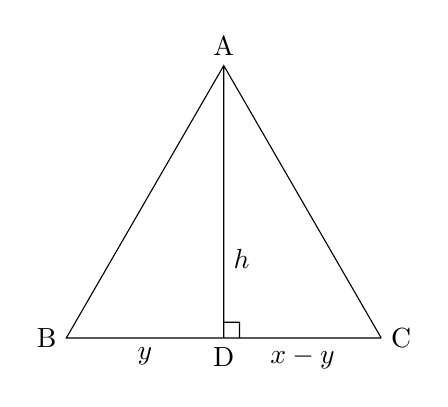
\begin{tikzpicture}
  \draw
    (4,0) coordinate (a) node[right] {C}
    -- (0,0) coordinate (b) node[left] {B}
    -- (2,3.46) coordinate (c) node[above] {A} -- (a)
    (2,0) coordinate (d) node[below] {D}
    (c) -- (d)
    (2,0.2) -- (2.2, 0.2) -- (2.2,0);
    \draw (1,0) node[below] {$y$};
    \draw (3,0) node[below] {$x-y$};
    \draw (2,1) node[right] {$h$};
\end{tikzpicture}
  \end{center}
\begin{proof}
  Let the foot of perpendicular be $D$. We proceed by contradiction. Suppose
  otherwise, then the two sections separated by the foot of perpendicular must
  be of different length, i.e., $y\neq x-y$. Then we must have
  \[y\neq x-y \implies y^{2}\neq(x-y)^{2} \implies y^{2}+h^{2}\neq(x-y)^{2}+h^{2}\]
  and by the Pythagorean Theorem, $y^{2}+h^{2}=AB^{2}$ and
  $(x-y)^{2}+h^{2}=AC^{2}$ gives us that
  \[y^{2}+h^{2}\neq(x-y)^{2}+h^{2}\implies AB^{2}\neq AC^{2}\implies AB\neq AC\],
  and this contradicts the assumption that fact that $AB=AC$. Therefore, we must
  have $AD=DC$ as desired.
  \end{proof}
\begin{claim}
  An equilateral triangle with side length $x$ has area $\frac{\sqrt{3}}{4}x^{2}$.
\end{claim}
\begin{center}
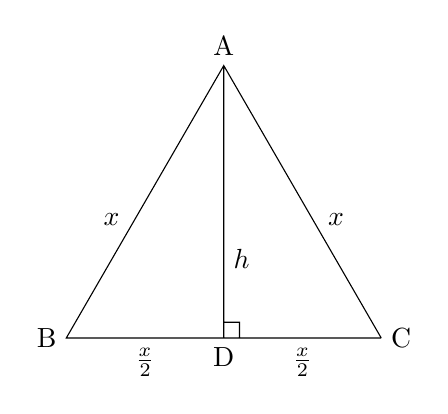
\begin{tikzpicture}
  \draw
    (4,0) coordinate (a) node[right] {C}
    -- (0,0) coordinate (b) node[left] {B}
    -- (2,3.46) coordinate (c) node[above] {A} -- (a)
    (2,0) coordinate (d) node[below] {D}
    (c) -- (d)
    (2,0.2) -- (2.2, 0.2) -- (2.2,0);
    \draw (1,0) node[below] {$\frac{x}{2}$};
    \draw (3,0) node[below] {$\frac{x}{2}$};
    \draw (0.8,1.5) node[left] {$x$};
    \draw (3.2,1.5) node[right] {$x$};
    \draw (2,1) node[right] {$h$};
\end{tikzpicture}
\end{center}
\begin{proof}
  Similarly, let $D$ be the foot of perpendicular of $A$ on $BC$, where $\triangle ABC$
  is equilateral. Our previous claim yields $BD=DC=\frac{x}{2}$ since $AB=AC$.
  By the Pythagorean Theorem, the length of $AD$, by considering either of
  $\triangle ABD$ or $\triangle ACD$ is
  \[
    \sqrt{x^{2} - (\frac{x}{2})^{2}} = \sqrt{\frac{3x^{2}}{4}} = \frac{\sqrt{3}x}{2}
  \]
  Therefore,
  \[
    \text{Area of }\triangle ABC = \frac{1}{2}\cdot BC\cdot AD = \frac{1}{2}(x)(\frac{\sqrt{3}x}{2}) = \frac{\sqrt{3}x^{2}}{4}
  \] as desired.
\end{proof}
Finally, with these 3 claims, we tackle the problem and show the area enclosed
by the two arcs $CAD$ and $CBD$ is
\[2r^{2}(\frac{\pi}{3} - \frac{\sqrt{3}}{a}),\ \text{where}\ a=4 \].
\begin{proof}
  Note that the desired area is equal to the sum of area of the four sectors:
  $ABC, BCA, ABD, BDA$ minus off the double-counted area, which is exactly the
  area of the quadilateral (rhombus) $ACBD$.\\
  Each of the four sectors have an angle of $60^{\circ}$ as seen from the
  equilateral triangles they contain. Since the two circles centered at $A$ and
  $B$ share a same radius $r$, all the sectors share the same area, that is
  $\frac{60^{\circ}}{360^{\circ}} = 1/6$ of the area of a circle with radius $r$. Four
  of these sectors contribute then to $4\cdot(1/6) = 2/3$ the area of a circle with
  radius $r$, namely $\frac{2}{3}\pi r^{2}$ in total.\\
  The area of the double-counted rhombus $ACBD$ is formed by two equilateral
  triangles, and therefore have an area of
  $\frac{\sqrt{3}r^{2}}{4}\times 2=\frac{\sqrt{3}r^{2}}{2}$.\\
  Taking the difference of the areas, the area enclosed by the arcs $CAD$ and
  $CBD$ is
  \[ \frac{2}{3}\pi r^{2}-\frac{\sqrt{3}r^{2}}{2}=2r^{2}(\frac{\pi}{3}-\frac{\sqrt{3}}{4})\]
  as desired.
\end{proof}                                                
\end{document}
